% !TEX program = xelatex

\documentclass[12pt,a4paper]{article}
\usepackage[UTF8]{ctex}
\usepackage{float}
\usepackage{amsmath}
\usepackage{amsfonts}
\usepackage{enumerate}
\usepackage{booktabs}
\usepackage{graphicx}
\usepackage{longtable}
\usepackage{subfigure}
\usepackage{multirow}
\usepackage{url}

% for plotting 
\usepackage{caption}
\usepackage{pgfplots}

% for pseudo code 
\usepackage{algorithm}
\usepackage[noend]{algpseudocode}

% for reference 
\usepackage{hyperref}
\usepackage{cleveref}
\crefname{equation}{方程}{方程}
\Crefname{equation}{方程}{方程}
\crefname{table}{表}{表}
\Crefname{table}{表}{表}
\crefname{figure}{图}{图}
\Crefname{figure}{图}{图}

% for code 
\usepackage{listings}
\usepackage{xcolor}
\usepackage{fontspec}
\definecolor{darkgreen}{rgb}{0,0.6,0}
\newfontfamily\consolas{Consolas}

\lstset {
    basicstyle=\footnotesize\consolas, % basic font setting
    breaklines=true, 
    frame=single,     % {single, shadowbox, bottomline}
    keywordstyle=\color{blue}, 
    commentstyle=\color{darkgreen},
    stringstyle=\color{red},
    showstringspaces=false,
    % backgroundcolor=\color{black!5}, % set backgroundcolor
    % numbers=left, 
    % numberstyle=\consolas,
}

% Microsoft Word A4 paper default layout 
\usepackage[a4paper, left=3.18cm, right=3.18cm, top=2.54cm, bottom=2.54cm]{geometry}

\captionsetup[figure]{labelfont={bf}, name={图}}
\captionsetup[table]{labelfont={bf}, name={表}}

\title{DIP Lab 3: Seam Carving}
\author{2017011620 \quad 计73 \quad 李家昊}
\date{\today}

\begin{document}

\maketitle

\section{Aspect Ratio Change}

对于图片宽高比的调整,这里采用了Seam Carving算法\cite{avidan2007seam}实现,不失一般性,可以仅实现对列的插入和删除,对行的操作可通过旋转图片实现,若行列均有变化,则先操作行,再操作列。

对于一张图片$\mathbf{I}$,计算它在每一个像素的能量,定义为,
\begin{equation}
    E(\mathbf{I}) = \left|\frac{\partial}{\partial x} \mathbf{I}\right| + \left|\frac{\partial}{\partial y} \mathbf{I}\right| 
\end{equation}
在具体实现中,$x,y$两个方向上的梯度是通过Sobel算子对图像进行卷积计算出来的,记,
\begin{equation}
    \mathbf{G}_x = \left(
    \begin{matrix}
        -1 & 0 & +1 \\
        -2 & 0 & +2 \\
        -1 & 0 & +1
    \end{matrix}
    \right),
    \quad
    \mathbf{G}_y = \left(
    \begin{matrix}
        -1 & -2 & -1 \\
        0 & 0 & 0 \\
        +1 & +2 & +1
    \end{matrix}
    \right)
\end{equation}
则图像的能量可表示为,
\begin{equation}
    E(\mathbf{I}) = |\mathbf{G}_x * \mathbf{I}| + |\mathbf{G}_y * \mathbf{I}|
\end{equation}

得到图像的能量后,可以通过动态规划,计算出从上往下到达每个位置$(i,j)$的缝的总计最小能量,
\begin{equation}
    \mathbf{M}(i,j) = E(i, j) + \min(\mathbf{M}(i-1,j-1), \mathbf{M}(i-1,j), \mathbf{M}(i-1, j+1))
\end{equation}
对矩阵$\mathbf{M}$进行回溯,即可得到能量最小的缝。这样一来,对图像宽度的压缩或扩展可通过缝的删除或增加来实现。需要注意的是,对于图像变窄,可以每次删除能量最小的一条缝,循环多次即可;而对于图像拓宽,则需要根据初始的能量,一次性选出所有待插入的缝,然后依次插入,插入像素取缝两边像素的均值。

实验结果如\Cref{fig:narrow},\Cref{fig:widen}所示,这里仅展示了列方向上的图像变窄和拓宽,对于行方向的操作,只需对图像旋转90度后进行列操作即可,这里不再展示。

\begin{figure}[H]
    \centering
    \subfigure[原始图像]{
        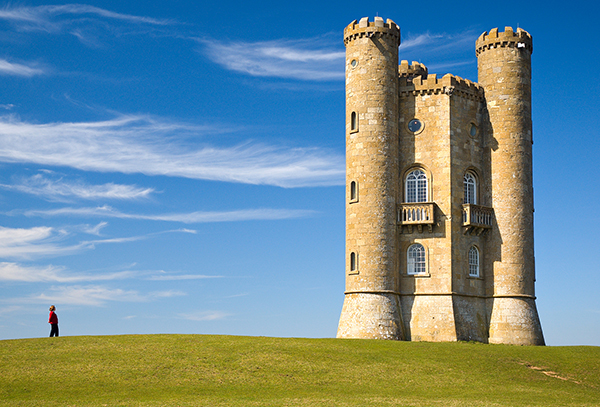
\includegraphics[height=4.5cm]{../fig/castle.jpg}
    }
    \subfigure[处理后]{
        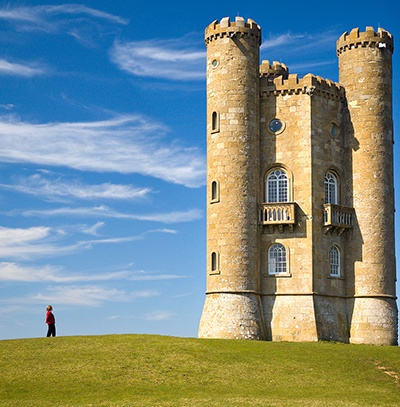
\includegraphics[height=4.5cm]{../output/castle.jpg}
    }
    \subfigure[原始图像的能量]{
        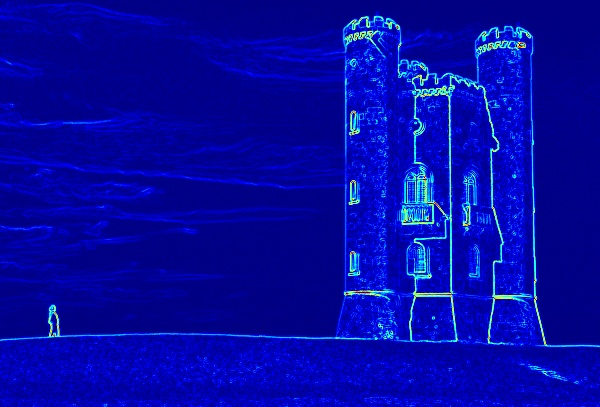
\includegraphics[height=4.5cm]{../output/castle_energy.jpg}
    }
    \subfigure[原始图像的总计最小能量]{
        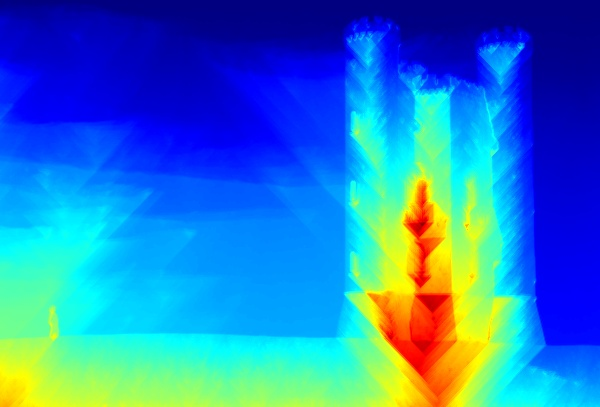
\includegraphics[height=4.5cm]{../output/castle_cost.jpg}
    }
    \caption{图像变窄}
    \label{fig:narrow}
\end{figure}

\begin{figure}[H]
    \centering
    \subfigure[原始图像]{
        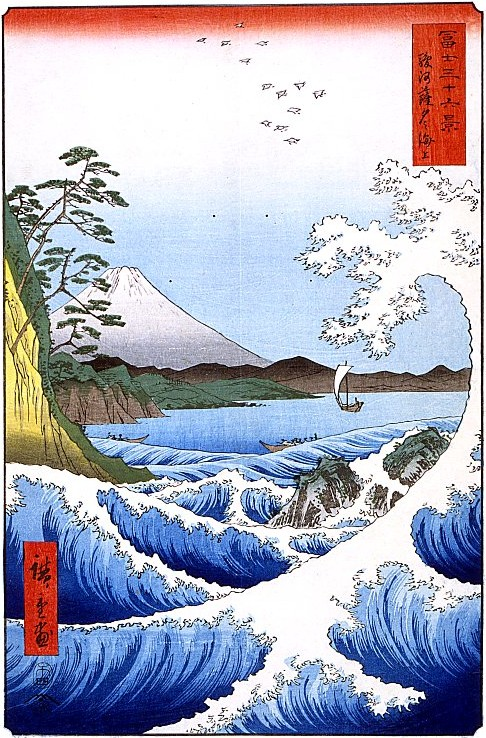
\includegraphics[height=4.4cm]{../fig/fuji.png}
    }
    \subfigure[处理后]{
        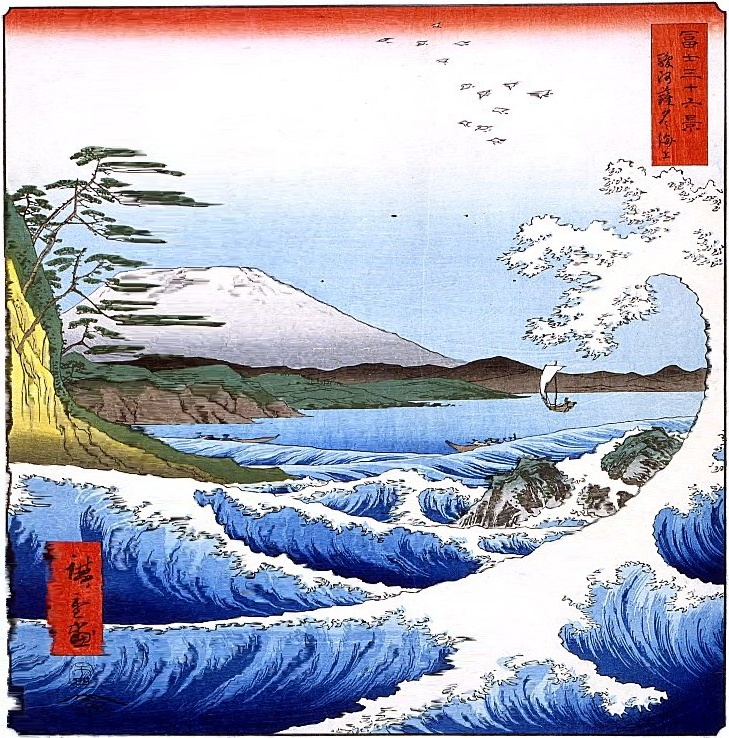
\includegraphics[height=4.4cm]{../output/fuji.jpg}
    }
    \subfigure[原始能量]{
        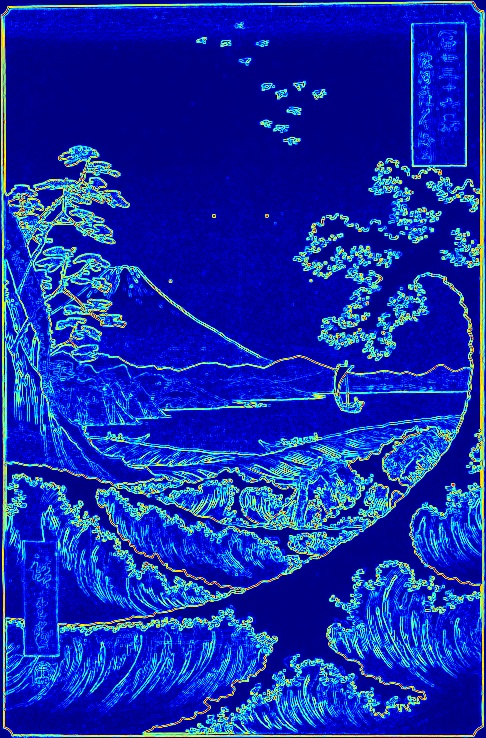
\includegraphics[height=4.4cm]{../output/fuji_energy.jpg}
    }
    \subfigure[总计最小能量]{
        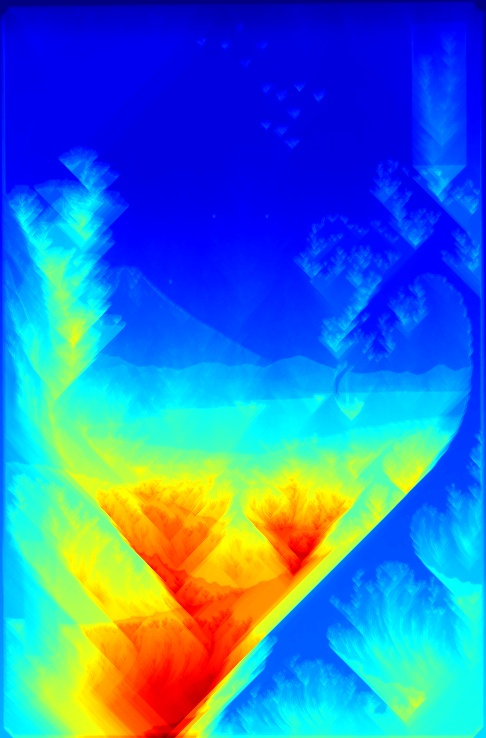
\includegraphics[height=4.4cm]{../output/fuji_cost.jpg}
    }
    \caption{图像加宽}
    \label{fig:widen}
\end{figure}

\section{Object Removal}

对于物体的删除,在每次计算能量时,将物体上像素的能量置为一个负值即可,使得每次最小能量的缝都通过物体,这样就可以高效地删除物体。实验结果如\Cref{fig:remove_object}所示,其中物体的分割可通过Photoshop处理得到,在去掉物体后,这里进一步采用Seam Carving的方法将图像拓宽为原始大小。

\begin{figure}[H]
    \centering
    \subfigure[原始图像]{
        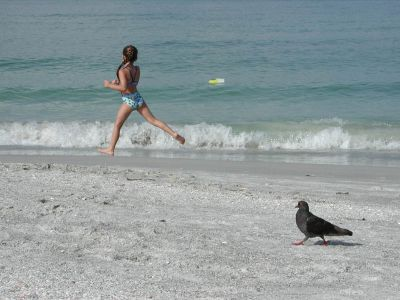
\includegraphics[width=0.3\textwidth]{../fig/beach.png}
    }
    \subfigure[鸽子的分割]{
        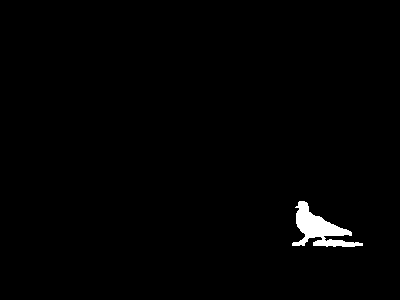
\includegraphics[width=0.3\textwidth]{../fig/beach_pigeon_mask.png}
    }
    \subfigure[女孩的分割]{
        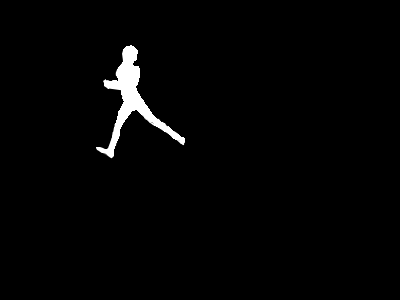
\includegraphics[width=0.3\textwidth]{../fig/beach_girl_mask.png}
    }
    \subfigure[去掉鸽子]{
        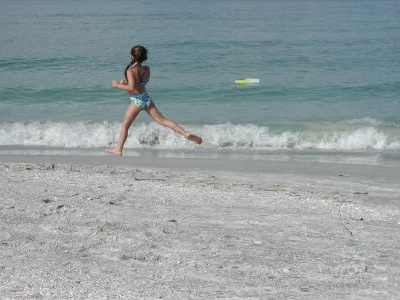
\includegraphics[width=0.3\textwidth]{../output/beach_pigeon_resized.jpg}
    }
    \subfigure[去掉鸽子的能量]{
        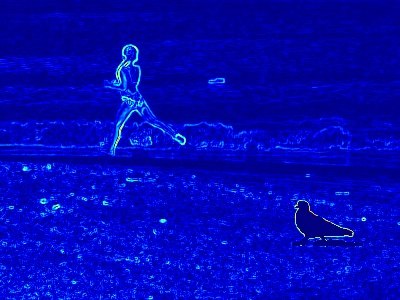
\includegraphics[width=0.3\textwidth]{../output/beach_pigeon_energy.jpg}
    }
    \subfigure[去掉鸽子的累计最小能量]{
        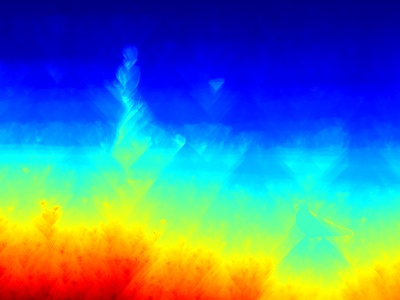
\includegraphics[width=0.3\textwidth]{../output/beach_pigeon_cost.jpg}
    }
    \subfigure[去掉女孩]{
        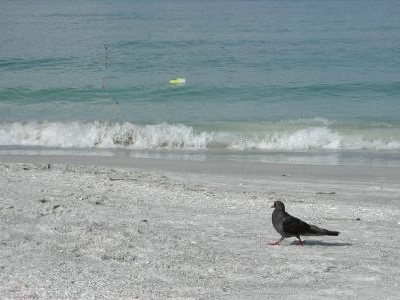
\includegraphics[width=0.3\textwidth]{../output/beach_girl_resized.jpg}
    }
    \subfigure[去掉女孩的能量]{
        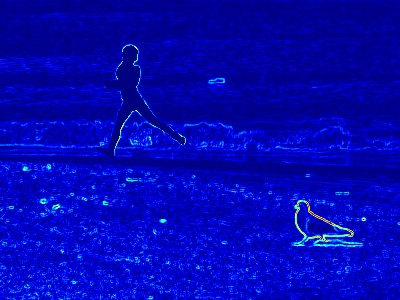
\includegraphics[width=0.3\textwidth]{../output/beach_girl_energy.jpg}
    }
    \subfigure[去掉女孩的累计最小能量]{
        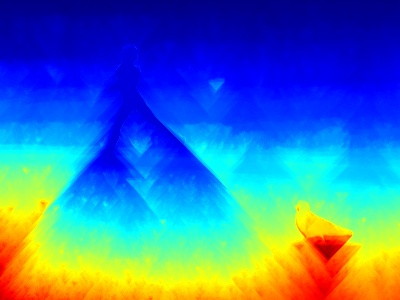
\includegraphics[width=0.3\textwidth]{../output/beach_girl_cost.jpg}
    }
    \caption{物体的删除}
    \label{fig:remove_object}
\end{figure}

\bibliographystyle{abbrv}
\bibliography{report}

\end{document}